\documentclass[12pt,preprint, authoryear]{elsarticle}

\usepackage{lmodern}
%%%% My spacing
\usepackage{setspace}
\setstretch{1.2}
\DeclareMathSizes{12}{14}{10}{10}

% Wrap around which gives all figures included the [H] command, or places it "here". This can be tedious to code in Rmarkdown.
\usepackage{float}
\let\origfigure\figure
\let\endorigfigure\endfigure
\renewenvironment{figure}[1][2] {
    \expandafter\origfigure\expandafter[H]
} {
    \endorigfigure
}

\let\origtable\table
\let\endorigtable\endtable
\renewenvironment{table}[1][2] {
    \expandafter\origtable\expandafter[H]
} {
    \endorigtable
}


\usepackage{ifxetex,ifluatex}
\usepackage{fixltx2e} % provides \textsubscript
\ifnum 0\ifxetex 1\fi\ifluatex 1\fi=0 % if pdftex
  \usepackage[T1]{fontenc}
  \usepackage[utf8]{inputenc}
\else % if luatex or xelatex
  \ifxetex
    \usepackage{mathspec}
    \usepackage{xltxtra,xunicode}
  \else
    \usepackage{fontspec}
  \fi
  \defaultfontfeatures{Mapping=tex-text,Scale=MatchLowercase}
  \newcommand{\euro}{€}
\fi

\usepackage{amssymb, amsmath, amsthm, amsfonts}

\def\bibsection{\section*{References}} %%% Make "References" appear before bibliography


\usepackage[round]{natbib}

\usepackage{longtable}
\usepackage[margin=2.3cm,bottom=2cm,top=2.5cm, includefoot]{geometry}
\usepackage{fancyhdr}
\usepackage[bottom, hang, flushmargin]{footmisc}
\usepackage{graphicx}
\numberwithin{equation}{section}
\numberwithin{figure}{section}
\numberwithin{table}{section}
\setlength{\parindent}{0cm}
\setlength{\parskip}{1.3ex plus 0.5ex minus 0.3ex}
\usepackage{textcomp}
\renewcommand{\headrulewidth}{0.2pt}
\renewcommand{\footrulewidth}{0.3pt}

\usepackage{array}
\newcolumntype{x}[1]{>{\centering\arraybackslash\hspace{0pt}}p{#1}}

%%%%  Remove the "preprint submitted to" part. Don't worry about this either, it just looks better without it:
\makeatletter
\def\ps@pprintTitle{%
  \let\@oddhead\@empty
  \let\@evenhead\@empty
  \let\@oddfoot\@empty
  \let\@evenfoot\@oddfoot
}
\makeatother

 \def\tightlist{} % This allows for subbullets!

\usepackage{hyperref}
\hypersetup{breaklinks=true,
            bookmarks=true,
            colorlinks=true,
            citecolor=blue,
            urlcolor=blue,
            linkcolor=blue,
            pdfborder={0 0 0}}


% The following packages allow huxtable to work:
\usepackage{siunitx}
\usepackage{multirow}
\usepackage{hhline}
\usepackage{calc}
\usepackage{tabularx}
\usepackage{booktabs}
\usepackage{caption}


\newenvironment{columns}[1][]{}{}

\newenvironment{column}[1]{\begin{minipage}{#1}\ignorespaces}{%
\end{minipage}
\ifhmode\unskip\fi
\aftergroup\useignorespacesandallpars}

\def\useignorespacesandallpars#1\ignorespaces\fi{%
#1\fi\ignorespacesandallpars}

\makeatletter
\def\ignorespacesandallpars{%
  \@ifnextchar\par
    {\expandafter\ignorespacesandallpars\@gobble}%
    {}%
}
\makeatother

\newenvironment{CSLReferences}[2]{%
}

\urlstyle{same}  % don't use monospace font for urls
\setlength{\parindent}{0pt}
\setlength{\parskip}{6pt plus 2pt minus 1pt}
\setlength{\emergencystretch}{3em}  % prevent overfull lines
\setcounter{secnumdepth}{5}

%%% Use protect on footnotes to avoid problems with footnotes in titles
\let\rmarkdownfootnote\footnote%
\def\footnote{\protect\rmarkdownfootnote}
\IfFileExists{upquote.sty}{\usepackage{upquote}}{}

%%% Include extra packages specified by user
\usepackage{booktabs}
\usepackage{longtable}
\usepackage{array}
\usepackage{multirow}
\usepackage{wrapfig}
\usepackage{float}
\usepackage{colortbl}
\usepackage{pdflscape}
\usepackage{tabu}
\usepackage{threeparttable}
\usepackage{threeparttablex}
\usepackage[normalem]{ulem}
\usepackage{makecell}
\usepackage{xcolor}

%%% Hard setting column skips for reports - this ensures greater consistency and control over the length settings in the document.
%% page layout
%% paragraphs
\setlength{\baselineskip}{12pt plus 0pt minus 0pt}
\setlength{\parskip}{12pt plus 0pt minus 0pt}
\setlength{\parindent}{0pt plus 0pt minus 0pt}
%% floats
\setlength{\floatsep}{12pt plus 0 pt minus 0pt}
\setlength{\textfloatsep}{20pt plus 0pt minus 0pt}
\setlength{\intextsep}{14pt plus 0pt minus 0pt}
\setlength{\dbltextfloatsep}{20pt plus 0pt minus 0pt}
\setlength{\dblfloatsep}{14pt plus 0pt minus 0pt}
%% maths
\setlength{\abovedisplayskip}{12pt plus 0pt minus 0pt}
\setlength{\belowdisplayskip}{12pt plus 0pt minus 0pt}
%% lists
\setlength{\topsep}{10pt plus 0pt minus 0pt}
\setlength{\partopsep}{3pt plus 0pt minus 0pt}
\setlength{\itemsep}{5pt plus 0pt minus 0pt}
\setlength{\labelsep}{8mm plus 0mm minus 0mm}
\setlength{\parsep}{\the\parskip}
\setlength{\listparindent}{\the\parindent}
%% verbatim
\setlength{\fboxsep}{5pt plus 0pt minus 0pt}



\begin{document}



\begin{frontmatter}  %

\title{Question 5}

% Set to FALSE if wanting to remove title (for submission)




\author[Add1]{Wesley James Williams}
\ead{21691126@sun.ac.za}





\address[Add1]{Stellenbosch University, South Africa}

\cortext[cor]{Corresponding author: Wesley James Williams}

\begin{abstract}
\small{
Currency volatiltiy analysis using GARCH methodologies.
}
\end{abstract}

\vspace{1cm}





\vspace{0.5cm}

\end{frontmatter}

\setcounter{footnote}{0}



%________________________
% Header and Footers
%%%%%%%%%%%%%%%%%%%%%%%%%%%%%%%%%
\pagestyle{fancy}
\chead{}
\rhead{}
\lfoot{}
\rfoot{\footnotesize Page \thepage}
\lhead{}
%\rfoot{\footnotesize Page \thepage } % "e.g. Page 2"
\cfoot{}

%\setlength\headheight{30pt}
%%%%%%%%%%%%%%%%%%%%%%%%%%%%%%%%%
%________________________

\headsep 35pt % So that header does not go over title




\hypertarget{volatility-of-the-zar}{%
\section{Volatility of the ZAR}\label{volatility-of-the-zar}}

\begin{tabular}{l|r|r}
\hline
Name & avg\_std\_dev & rank\\
\hline
Ghana & 0.0133703 & 1\\
\hline
Argentina & 0.0119544 & 2\\
\hline
Nigeria & 0.0114748 & 3\\
\hline
Egypt & 0.0111624 & 4\\
\hline
Zambia & 0.0108368 & 5\\
\hline
Brazil & 0.0107192 & 6\\
\hline
Turkey & 0.0102997 & 7\\
\hline
SouthAfrica & 0.0101896 & 8\\
\hline
Russia & 0.0098690 & 9\\
\hline
Columbia & 0.0084828 & 10\\
\hline
Mexico & 0.0083886 & 11\\
\hline
Norway & 0.0073514 & 12\\
\hline
Chile & 0.0067539 & 13\\
\hline
NZ\_Inv & 0.0064288 & 14\\
\hline
Hungary & 0.0063517 & 15\\
\hline
Poland & 0.0062783 & 16\\
\hline
Australia\_Inv & 0.0061457 & 17\\
\hline
UK\_Inv & 0.0060173 & 18\\
\hline
Sweden & 0.0059233 & 19\\
\hline
Czech & 0.0057921 & 20\\
\hline
\end{tabular}

The table above ranks countries by their currencies average volatility,
measured by the average scaled dlog returs standard deviation, since
2018 and it shows that the South Afican ZAR has been the 8th most
volatile currency. But this may be due to noise.

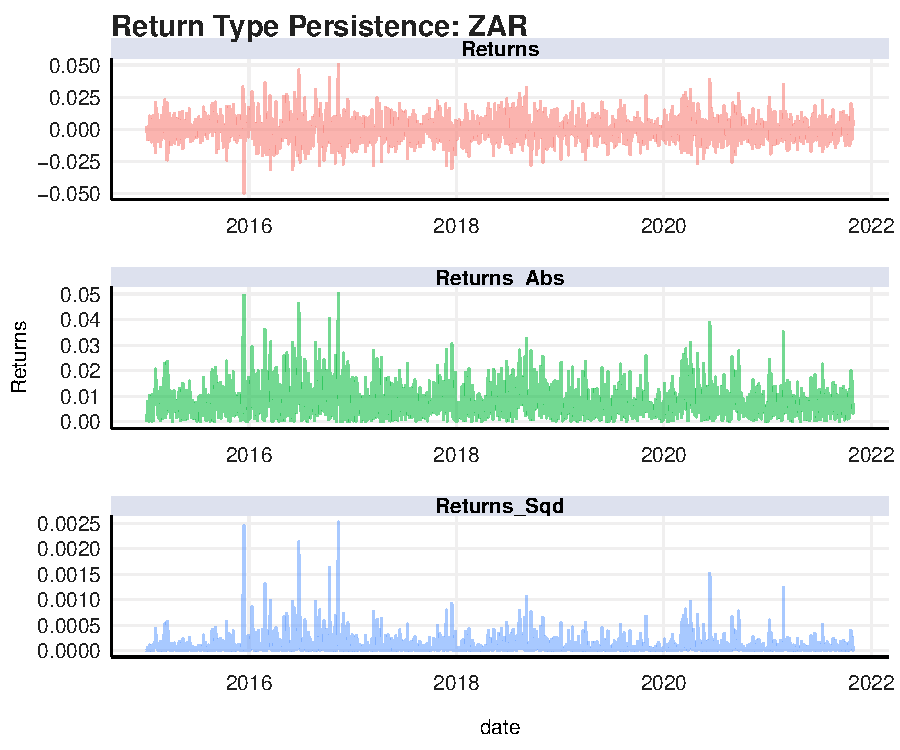
\includegraphics{Question-5_files/figure-latex/unnamed-chunk-3-1.pdf}
The figure above shows clear signs of both first and second order
persistence. To verify this I plot the ACFs.

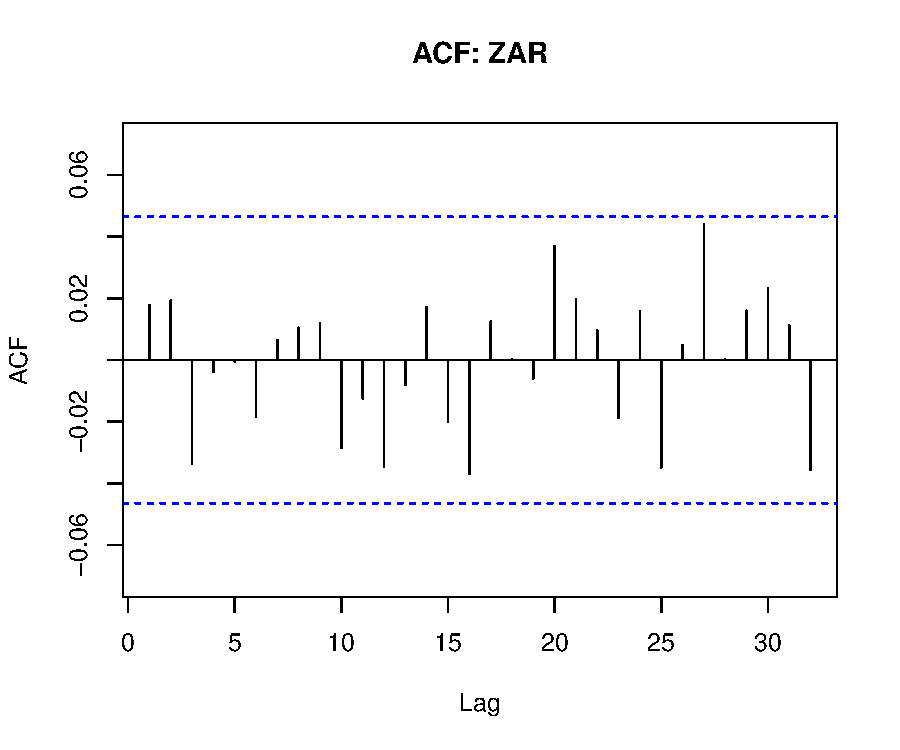
\includegraphics{Question-5_files/figure-latex/unnamed-chunk-4-1.pdf}

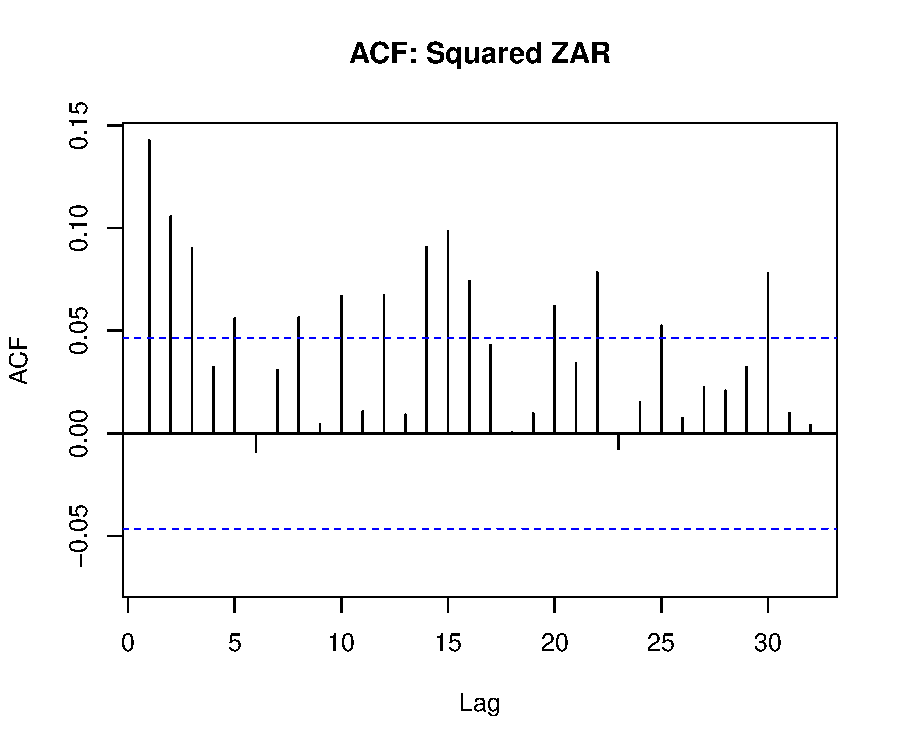
\includegraphics{Question-5_files/figure-latex/unnamed-chunk-5-1.pdf}

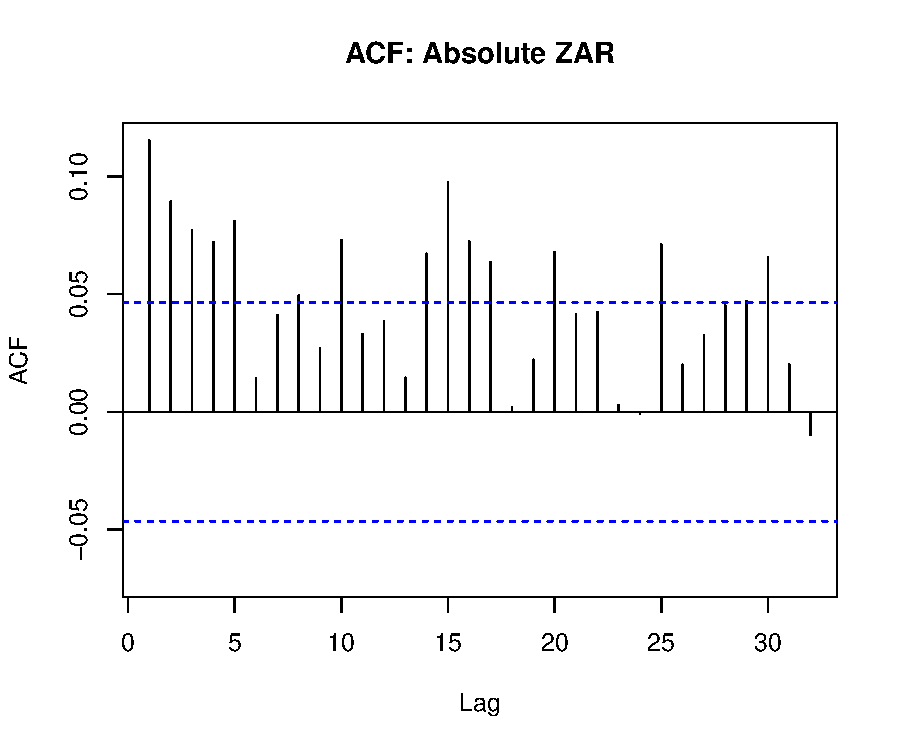
\includegraphics{Question-5_files/figure-latex/unnamed-chunk-6-1.pdf}

\begin{verbatim}
## 
##  Box-Ljung test
## 
## data:  coredata(zar_rts^2)
## X-squared = 101.98, df = 12, p-value = 2.22e-16
\end{verbatim}

Both the ACFs and the Box-Ljung test confirm that there is strong
conditional heteroskedasticity, as well as long memory. The null
hypothesis of no ARCH effects is rejected by the small p-value. \#\#
Fitting the GARCH

\begin{tabular}{l|r|r|r|r}
\hline
  &  Estimate &  Std. Error &  t value & Pr(>|t|)\\
\hline
mu & 0.0001290 & 0.0002892 & 0.4462246 & 0.6554350\\
\hline
ar1 & 0.0032466 & 0.0325598 & 0.0997119 & 0.9205730\\
\hline
omega & 0.0000029 & 0.0000009 & 3.1998093 & 0.0013752\\
\hline
alpha1 & 0.0454413 & 0.0050295 & 9.0348775 & 0.0000000\\
\hline
beta1 & 0.9224490 & 0.0107290 & 85.9768476 & 0.0000000\\
\hline
\end{tabular}

The alpha and beta coefficients are highly significant. This means that
there is strong persistence in volatility and of volatility clustering,
meaning periods of high volatility tend to follow each other.
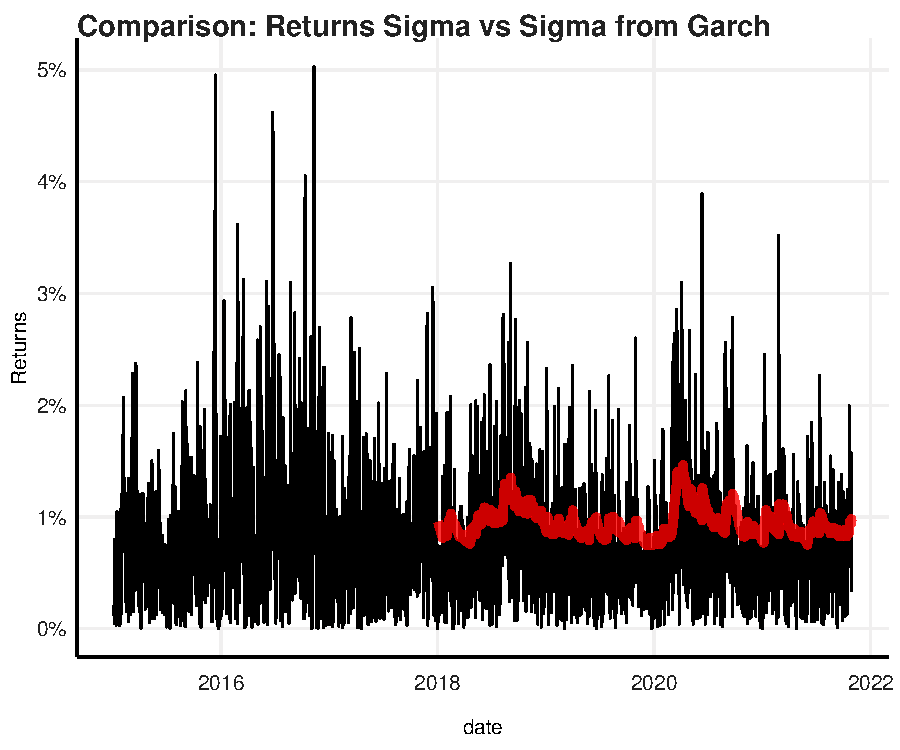
\includegraphics{Question-5_files/figure-latex/unnamed-chunk-10-1.pdf}
Now, we have a noise reduced measure of volatility.

\hypertarget{go-garch}{%
\subsection{GO-GARCH}\label{go-garch}}

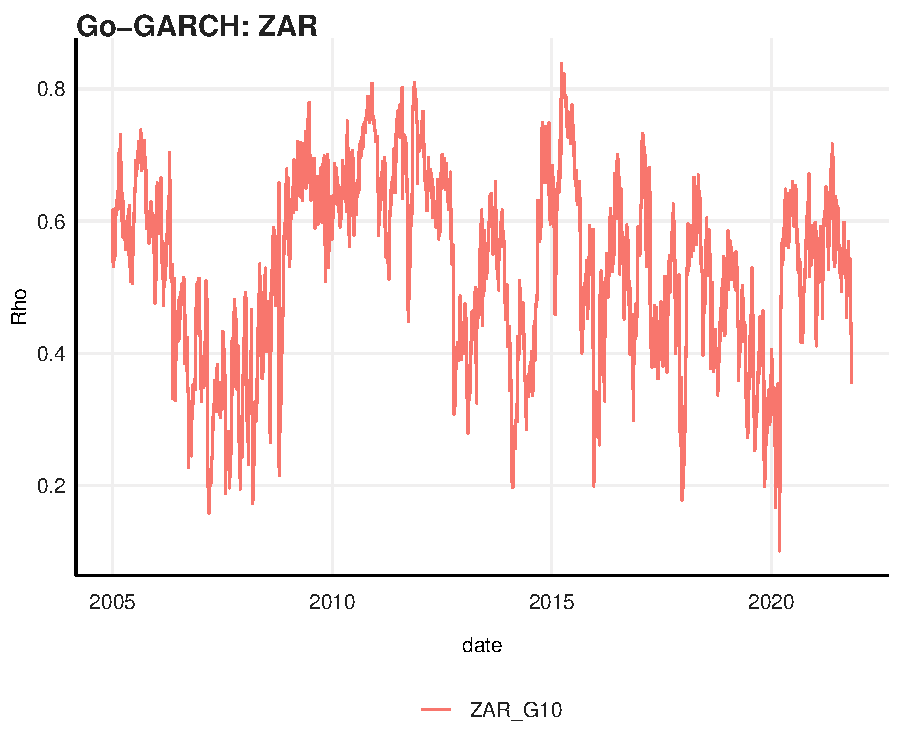
\includegraphics{Question-5_files/figure-latex/unnamed-chunk-12-1.pdf}
Lastly I plot the GO-GARCH's correlation between G10 currencies and the
Rand. This graph now provides more evidence for how volatile the Rand is
with the correleations over just 3 years ranging between 0.7 and 0.2.
\newpage

\hypertarget{references}{%
\section*{References}\label{references}}
\addcontentsline{toc}{section}{References}

\hypertarget{refs}{}
\begin{CSLReferences}{0}{0}
\end{CSLReferences}

\bibliography{Tex/ref}





\end{document}
